\documentclass[a4paper,12pt]{article}

\usepackage{url}
\usepackage{epsfig}
\usepackage{graphics}
\usepackage{fancyhdr}
\usepackage[parfill]{parskip} % Activate to begin paragraphs with an empty line rather than an indent
\usepackage{amsmath}
\usepackage{natbib}
\usepackage{subfigure}
\usepackage{svg}
\graphicspath{{pictures/}}

% SVG Options
\setsvg{inkscape = inkscape -z -D}
\setsvg{svgpath = pictures/}

\title{Carl Bildt Tweets: A comparison of regular and constrained Markov chain for text generation}
\author{\hspace*{-0.5cm}
Group Ain't intelligent\\
\begin{tabular}{cccc}
Viktor Bj\"{o}rkholm & Jesper Br\"{a}nn & Daniel Duberg & Jakob Tidestr\"{o}m\\
92-11-17 & 92-09-30 & 93-01-17 & 90-10-04 \\
viktorbj@kth.se & jbrann@kth.se & dduberg@kth.se & jakobti@kth.se \\
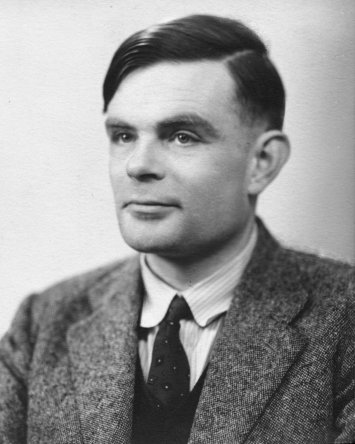
\includegraphics[width=0.13\linewidth]{Alan_Turing_photo} & 
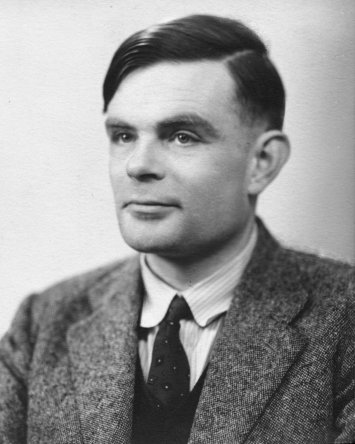
\includegraphics[width=0.13\linewidth]{Alan_Turing_photo} & 
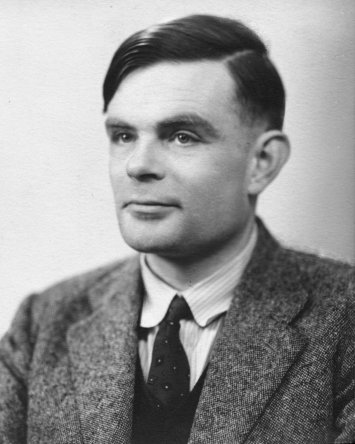
\includegraphics[width=0.13\linewidth]{Alan_Turing_photo} & 
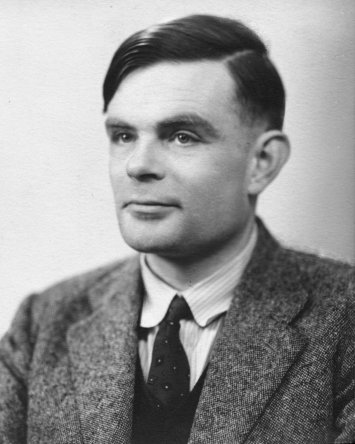
\includegraphics[width=0.13\linewidth]{Alan_Turing_photo}
\end{tabular}} 
% Normally there will not be any pictures but we want
% these so that we can connect faces to names in the course
% We also want birthdates so that we can tell people with the same
% name apart
\date{}

\pagestyle{fancy}
\setlength{\headheight}{15pt}
\fancyhf{}
\lhead{DD2380 ai14} % DO NOT REMOVE!!!!
\rhead{V. Bj\"{o}rkholm, J. Br\"{a}nn, D. Duberg, J. Tidestr\"{o}m} %% UPDATE WITH YOUR NAMES

\begin{document}

\maketitle
\thispagestyle{fancy}

\begin{abstract}
Skriv sist, när vi vet vad vi har skrivit om (y)
\end{abstract}



\clearpage

%%%%%%%%%%%%%%%%%%%%%%%%%%%%%%%%%%%%%%%%%%%%%%%%%%%%%%%%%%%%%
%%%%%%%%%%%%%%%%%%%%%%%%%%%%%%%%%%%%%%%%%%%%%%%%%%%%%%%%%%%%%
\section{Introduction (1--2 pages)}
\label{sec:intro}
% What is the problem and why is it important? 
% What will the reader get out of it? 
% Present specific results
% Dont go into detail 
This paper aims to develop an understanding on refining natural language text generation.
Natural Language Generation (NLG) is an area of research within the field of Artificial Intelligence. 
The purpose of NLG is to generate text that is semantically correct in order to make communication with computer systems more natural and understandable for users.

Within this paper we show the difference in quality of two different approaches to text generation. 
One of these approaches is using Markov chains or more commonly known as n-grams. 
These n-grams take n words in sequence and uses a corpus of text to guess what the most probable next word is. 
Using a larger n in an n-gram means that more text is copied straight from the corpus, 
however this also means that there is a higher likelihood that the text being generated is meaningful. 
% Givet att corpus är meningsfullt
We will contrast this method with using constrained Markov chains. 
The main constraint of the Markov chains is that two words following each other will have the same sequence of part-of-speech as the corpus.
Part-of-speech is a concept within NLG that divides a text into the different linguistical categories of the words within it.

We aim to show that using this constraint upon the Markov chain, sentences will have a greater diversity but still be as semantically correct as just using a n-gram.
Since the problem with larger n:s within n-grams is that text is copied straight from the corpus, 
the constraint will hopefully help us create semantically correct sentences with a greater diversity from the corpus.

To be able to show differences in these two approaches we generate Twitter messages, so called tweets. 
We build upon the work by \cite{shannon48} for the theory of implementing an n-gram, a description on generating and parsing corpuses by \citep{Corpus}
and the work by \citealp{McBarb} to implement our own constraints on the n-gram.
   
\subsection{Contribution}
% Förklara för en datalog varför det vi gjort ar vettigt.

We have implemented a unigram of part-of-speech (POS) on to a bigram in order to observe the difference in the result. 
As mentioned above a problem with n-grams with to high n:s is that they will simply copy parts of the corpus if said corpus does not contain a large variation of similar sentences, 
so that a given start of n words does not automatically lead to one sentence finish. i.e. a larger corpus is needed for larger n:s.
To be able to keep a smaller and diverse corpus we applied the unigram of POS tags on top of the n-gram to allow the program to select words of a common word type order and with a greater diversity than naturally occurs in the corpus.

Our main contribution to the field is that we have tried putting this unigram constraint upon the regular Markov chain and doing it for short message generation.
The research area we base this paper on focus on generating text that fits a theme or rhythm whereas we generalize the concept by creating text that is not constrained by a pre-written sequence of POS. 
Our approach is that we let the model be trained with two types of information, thus our contribution to the field lies in examining how the combination of these two approaches improves the general natural language generation.


%A lot new research involves the constraining of Markov chains to produce text that fits different molds than just text generated from a corpus. 
%It is important to be able to generate text that is 

\subsection{Outline}
We bring up the relation of our work to some other work in the field. \cite{McBarb} in section~\ref{sec:relwork} and explain how that research has affected ours. 
In section~\ref{sec:method} we then go through the details on how the algorithm works, 
we also give examples to explain in detail what the difference between the two methods we are comparing. This is complemented with details regarding our specific
implementation of the algorithm ni section~\ref{sec:impl}. The data from running the algorithm is explained, reviewed and evaluated in section~\ref{sec:exps}.

\newpage
%%%%%%%%%%%%%%%%%%%%%%%%%%%%%%%%%%%%%%%%%%%%%%%%%%%%%%%%%%%%%
%%%%%%%%%%%%%%%%%%%%%%%%%%%%%%%%%%%%%%%%%%%%%%%%%%%%%%%%%%%%%
\section{Related work (1--3 pages)}
\label{sec:relwork}
% It is here we show that we know the field well and present the reports that we have read
%% Saker vi behöver svara på i detta stycke:
% Vad vet vi om hur dem använde constraints i sitt arbete? Vi verkar ju inte veta något om det eftersom vi bara gissar oss fram :D
%
% Har vi något mer att basera vårat arbete på? En vetenskaplig text är ju bra, men om vi läst fler så är ju det rätt bra.

% Jesper skriv under härate sentenses from words.
In \cite{shannon48} Shannon goes through the first basic steps in how to naively generate text from a corpus with Markov chains. 
He explains in depth how Markov chains can be used to generate real sounding English words from letters and also sentences from words. 
By creating differently sized n-grams for both letters and words he shows how the results improve when n grows. 
The technique is building up a transition matrix where each row and column index are the words or letters that represent the states. 
The values of the rows in a column represent the probability of moving from the state of the column to the state of the row. 
The probabilities of the transitions between the different states is taught to the transition matrix by iterating through the corpus.
In a unigam the states could be every single different word and the probability of moving to one word from another is determined only by looking at the preceeding one.
However, in a bigram the different states grows exponentially as they could be every two combinations of represented sequences of word, 
since every new word in a bigram is dependent on the two preceeding ones.
This is then followed through to generate the text.
His approach was novel at the time but it is a staple in modern text generation. 
% Här kan vi lägga till massa content om vad det faktiskt innebär i praktiken vad dooden har gjort.
% Här kan vi förklara hur det relaterar till vad vi har gjort.
The base Markov chain used in this paper is generated in a similar way to what Shannon describes. 
It builds what is the ground of the algorithm which we build on to.


% Nisse skriv under här
In the work by \cite{Corpus}, they describe the process of building a corpus for a natural language generation system. 
Different steps are presented which span over the very basic demands such as the structure of the content of the corpus that is supposed to be examples of output. 
To clarify, the content of the corpus should be examples of what we want the output from our system to immitate. 
We applied this demand by populating our corpus with content in the same style that we want to generate. % Alltså känns typ dumt att skriva, men vi ska väl relatera till hur vi använt dem? Så, det här blir ju en rad extra...
They also describe an early step of deciding a form of constraints (user requerments) of the corpus, 
if the users want the output to maintain a specific format or if they want the output to exclude specific content.
As we play the role of our own users, we made sure to specify what kind of content we want to exclude that was naturally included in the corpus, 
such as hash-tags and image links in our case with tweets. % Här spoilar jag på något vis vad vi håller på med. Tweets!
Lastly it describes the step of applying the user requests on the collected data that we want to populate our corpus with.
It involves modifying, simplifying and removing data that we can not use in its original form.
We wrote a script that downloaded tweets in to our corpus that applied our requests on the format of the outputs on the data downloaded.
% Vad jag saknar i detta stycke:
% Jag ger antagligen credit till fel person, eftersom denne inte är upphovsman till allt detta.
% 

Our work on actually constraining Markov models is built upon \cite{McBarb} work, 
where the authors generated lyrics from different artists using Markov models with constraints. 
These were to be generated in a specific style and with a rhythm, to simulate real lyrics from a large span of artists.
They start in a standard fashion by building up a corpus of content that they want to imitate. 
In their case they built up a corpus consiting of the collected work of each artist. 
So when generating lyrics for bob dylan as an example, the corpus consisted of 7600 uniqe words, a total of 96 089 words and 12 408 verses.
They proceeded with applying constraints on a bigram to meet their demands on the generated text to have a certain style and to rhyme.
Some of the constraints they apply on their bigram is that some words need to have the same meter as in the original song, but also that the text generated
needs to fit a part-of-speech template and a rhytmic template that comes from the song the newly generated lyrics is to be based on. 
The templates are not generated by their algorithm, but rather handcrafted to get a proper result. Our take from this paper was to be able to apply constraints
upon a bigram, or rather a Markov chain in general. Similarily we utilize a part-of-speech template of sorts, but we diverge a bit from this paper.





\newpage

%%%%%%%%%%%%%%%%%%%%%%%%%%%%%%%%%%%%%%%%%%%%%%%%%%%%%%%%%%%%%
%%%%%%%%%%%%%%%%%%%%%%%%%%%%%%%%%%%%%%%%%%%%%%%%%%%%%%%%%%%%%
\section{My method (1--4 pages)}
\label{sec:method}
Our method that forms the basis of this paper is generating Twitter messages with the use of both Markov chains and constrained Markov chains and to compare the two methods with each other.
The theory is that constraining an Markov chain will yield better and more diverse text being generated. 
In section~\ref{sec:exps} where we explain our experiments and data we try out different orders of the Markov chain, 
for the sake of explanation we assume a first order Markov chain is used to explain how the method works. 
In a limited corpus such as this one: \\

\begin{tabular}{r | l}
``Rolf has a dog.`` & Noun $\to$ verb $\to$ singular quantifier $\to$ noun \\
``Rolf owns a dog.`` & Noun $\to$ verb $\to$ singular quantifier $\to$ noun \\
``Rolf can not walk his dog.`` & Noun $\to$ modal $\to$ adverb $\to$ verb $\to$ pronoun $\to$ noun \\
\end{tabular}

This corpus generates a Markov chain that looks like figure 1a, with the edges being the probabilities for the specific transitions. 
In the figure the specific part-of-speech is included in the states beneath the words from the corpus. 
If we then add constraints from a transition matrix, built up from POS-analysis of the same corpus we are given the new chain that is seen in figure 1b.

\begin{figure}[h!]
  \hfill
  \subfigure[Unigram of the limited corpus]{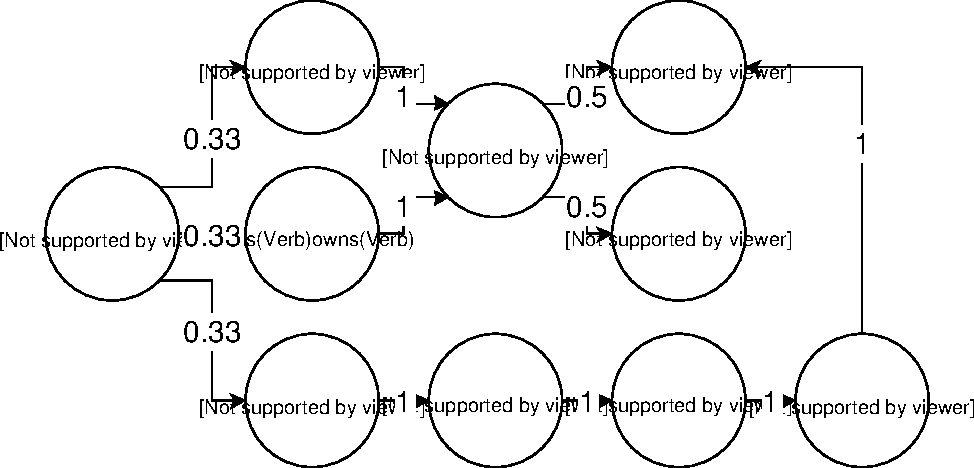
\includegraphics[width=0.49\linewidth]{Bigram.pdf}}
  \hfill
  \subfigure[Unigram with constraints applied]{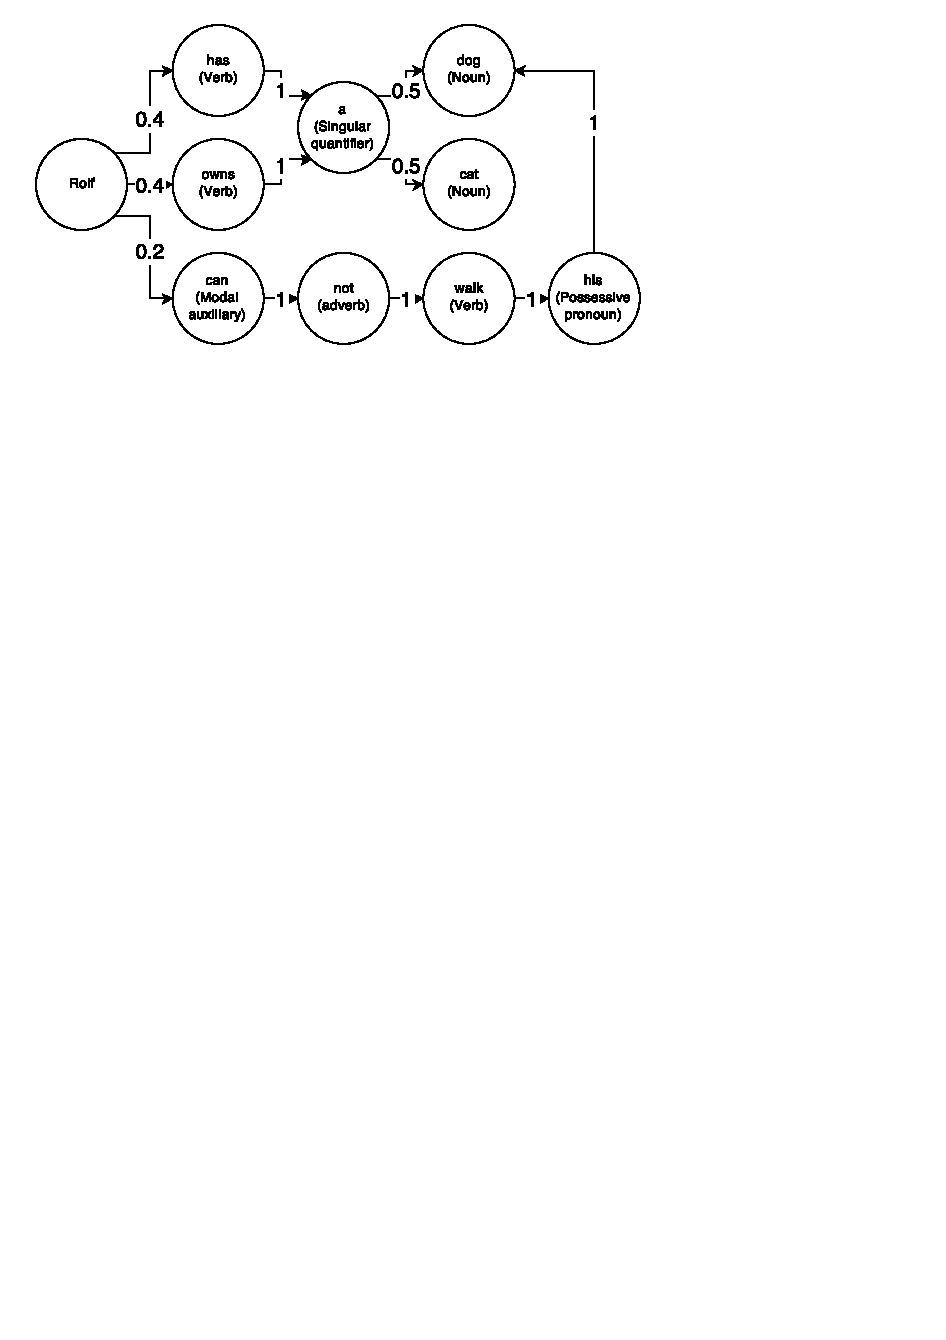
\includegraphics[width=0.49\linewidth]{Bigram2.pdf}}
  \hfill
  \caption{Unigrams}
 \end{figure}



We can see in figure 1b that since both ''has`` and ''owns`` are verbs they are more probable to occur than ''can``, this is reflected in the new edges. 
This happens because the part-of-speech ''verb`` is more likely to follow NNP according to our transition matrix, and thus ''has`` and ''owns``, who are 
both verbs become even more likely to follow NNP (Rolf). This method can then be further applied to a bigram, a trigram or any n-grams that follows. 
Our method however will only have an unigram for the transition matrix, even if the Markov chain of words from the corpus is longer, 
the transitions are only observed with one previous state in consideration.

\subsubsection{Calculating uniqueness}
We originally wanted to analyse the semantic correctness of our tweets but were unable to find a method of doing so mechanically. In lieu of other options we decided to instead analyse how unique the tweets were in terms of how much it just copied straight out of the corpus.

Since we use a bigram it will always take three successive words but anything above that compromises uniqueness.

For example purposes we added these sentences to the limited corpus mentioned earlier:

\begin{tabular}{l}
``Mufasa is a dog with a purple tail.``\\
``Mufasa owns a yellow cat.``\\
``Jessica can not eat a yellow dog with a pink tail.``\\
``Steve has a shirt with a purple tail.``\\
\end{tabular}

% Räkna manuellt med limited corpus
\textbf{Example 1:} ``Rolf can not eat a yellow cat.``
	
It first matches "can not eat a yellow" since it is the largest continuous match, this reduces uniqueness by 2. What is left is "Rolf" and "cat" since both are shorter than three words we stop here.

Thus this sentences uniqueness is $\frac{9 - 2}{9} \approx$ 78\%.

\textbf{Example 2:} ``Rolf has a shirt with a yellow dog with a pink tail.``
	
The first match is "a yellow dog with a pink tail", reducing uniqueness by 4. Remaining is "Rolf has a shirt with" which matches "has a shirt with", further reducing uniqueness by 1. Only "Rolf" is left over thus we stop. 

Thus this sentence has a uniqueness of $\frac{12 - (4 + 1)}{12} \approx$ 58\%.

\subsubsection{Corpus}
In order to generate tweets, we first discussed the problem regarding the semantical corectness of a generalized tweet.
The average level is according to our own experience far from sematically correct, which isn't a problem in understadabillity for an experienced Twitter user,
but is a problem for our POS who would not recognize the words. Even if it would give it an ''unknown``-tag, we would not be able to predict any kind of results.

\begin{figure}[h!]
  \centering
  
\includegraphics[width=1\linewidth]{machine_learning}
  \caption{An example tweet}
\end{figure}

To solve this problem approximatily, we decided to generate tweets for a specific user who mostly uses correct grammar and semantics when tweeting and tweets in English.
Our option fell on Carl Bildt, former foreign minister of Sweden, because of his active use of Twitter, 
that he tweets in English and that most of his tweets are in grammatically correct English.

\subsection{Implementation (0--2 pages)}
\label{sec:impl}
The implementation relied on a Part-of-Speech tagger from Stanford's Natural Language Processsing group.

We start by collecting data, in the form of tweets, by a target person, Carl Bildt, to be used as the corpus of our tweet generator. The data is filtered to remove unwanted elements such as hashtags and web addresses.

Each tweet is run through Stanford's speech tagger to get the lexical class of each word depending on context.
We then use these lexical classes as states for the transition matrix, more specifically they're used to see what lexical class usually follows any given lexical class or terminates a sentence.

While iterating through the gathered data we store what word follows any given two words, including sentence terminating symbols such as '.' or '!' and store it as a bigram.

When generating tweets two methods are used, first the bigram gets to select which words to use entirely on its own digression (Markov chain). Then the process is repeated but this time the bigram is constrained by which lexical class of words it is allowed to choose from, that class being whichever one the transition matrix has decided should follow (constrained Markov chain).

%%%%%%%%%%%%%%%%%%%%%%%%%%%%%%%%%%%%%%%%%%%%%%%%%%%%%%%%%%%%%
%%%%%%%%%%%%%%%%%%%%%%%%%%%%%%%%%%%%%%%%%%%%%%%%%%%%%%%%%%%%%
\section{Experimental results (1--4 pages)}
\label{sec:exps}

\subsection{Experimental setup}
We generate 10000 tweets with a length of between 30 and 140 characters using both the Markov chain and the constrained Markov chain.

Once generated we analyse the tweets uniqueness by counting how many of the used words are from the same part of the corpus. However, since we use a bigram three of the words have to appear in succession and thus we only count if four or more of the words are from the same part of the corpus. We then divide this by the number of words to get an average for the whole tweet.

\subsection{Experiment}

\subsubsection{Uniqueness based on words in tweet}

\begin{figure}[h!]
  \hfill
  {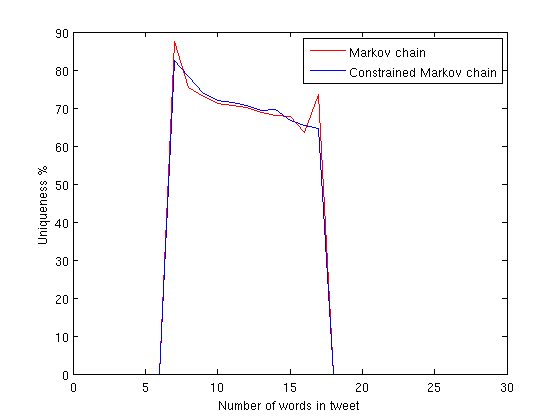
\includegraphics[width=1\linewidth, height = 200]{UniqByNumWordsTweet.png}}
  \caption{Uniqueness based on words in tweet}
 \end{figure}
 
 \begin{figure}[h!]
   \hfill
  {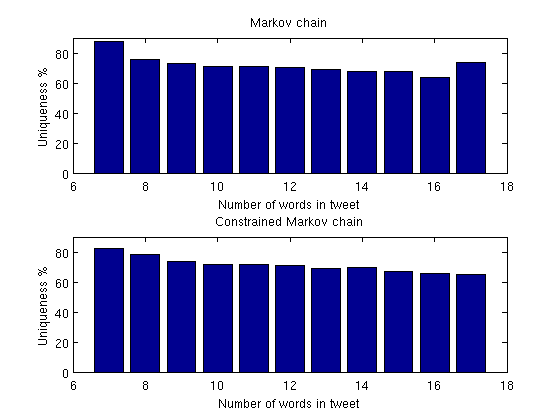
\includegraphics[width=1\linewidth, height = 200]{UniqByNumWordsTweet2.png}}
  \hfill
  \caption{Uniqueness based on words in tweet (Comparison)}
 \end{figure}
 
 Uniqueness drops as the number of words in the tweet increases
 % Unikhet minskar när längd ökar men de har lika värden, förutom de spikes som markov kedjan får i början och slutet

\newpage

\subsubsection{Number of tweets based on uniqueness}
% Även här lika, markov chain har mer värden som har låg unikhet än constrained och markov chain har fler värden som har hög unikhet

\subsubsection{Actual content of tweet}
% Jämför TM och utan och se vilka som genererar bäst tweets att läsa/förstå.

\newpage
%%%%%%%%%%%%%%%%%%%%%%%%%%%%%%%%%%%%%%%%%%%%%%%%%%%%%%%%%%%%%
%%%%%%%%%%%%%%%%%%%%%%%%%%%%%%%%%%%%%%%%%%%%%%%%%%%%%%%%%%%%%
\section{Summary and Conclusions (0.5--1 page)}
\label{sec:summary}
% Vad har vi kommit fram till?
We compared generating natural language with a native bigram from our corpus with using a constrained markov chain with a bigram to generate tweets seeming to origin from a specific user.
In the result we can see that using a constrained markov chain has a slight advantage over simply using a bigram in generating a diversity of content. % Behövs diskussion om hur pass de verkade vara från CB himself.
% Vad bidrog det med?
We were able to show that with a slight change in implementation we could slightly change the outcome of results. 
% Hur kan våra resultat förbättras/förändras?
The constrained matrix only uses a unigram, if it would use a bigram for it's POS constraints, perhaps the outcome would have been different. Or less diversity. What do we know. We need logic here.
Using i bigram for constraints would perhaps give a more stable result and thus beeing more similar to only using a bigram. But since it's POS, i have no idea.s

%%%%%%%%%%%%%%%%%%%%%%%%%%%%%%%%%%%%%%%%%%%%%%%%%%%%%%%%%%%%%
%%%%%%%%%%%%%%%%%%%%%%%%%%%%%%%%%%%%%%%%%%%%%%%%%%%%%%%%%%%%%
\bibliographystyle{plainnat}
\bibliography{reflist}


\end{document}